% Auteur: Mischa Masson, basé sur le travail de Nicolas Englebert (Mise en forme) et Enes Ulusoy(contenu,images)
\documentclass[british,french,11pt, a4paper, openany]{article}

%%%%%%%%%%%%%%%%
%%% Packages %%%
%%%%%%%%%%%%%%%%

%%% Général %%%
\usepackage[utf8]{inputenc}   
\usepackage[french]{babel}
\usepackage[T1]{fontenc}
\usepackage{mathpazo}
\usepackage{lmodern}
\usepackage{courier}
\usepackage{graphicx}
\usepackage{cancel}

%%% Tableau %%%
\usepackage{tabularx} %Permet d'auto dimensionner les tableaux



%%% Bibliographie %%%
\usepackage[style=alphabetic,backend=bibtex]{biblatex}
\usepackage[autostyle]{csquotes}
\DeclareNameAlias{sortname}{last-first}
\DeclareFieldFormat{url}{\space\url{#1}}
\DeclareNameAlias{labelname}{last-first}
\addbibresource{sample.bib}


%%% Graphiques %%%
\usepackage{tikz}
\usepackage{pgfplots}
\usepackage{circuitikz}

%%% Mise en page %%%
\usepackage{amsmath}
\usepackage{amsfonts}
\usepackage{amssymb}
\usepackage{amsthm}
\usepackage[tt]{titlepic}% Centre le titre
\usepackage{fancyhdr}   % Permet de modifier l'entête & footer
\usepackage{caption}     % Permet d'ajouter des légendes en images sans les mettre en float + dans la marge + ref vers le haut de l'envirronement
\usepackage{wrapfig}
\usepackage{fullpage}
\usepackage{multicol}   % pour les liste sur plusieurs colonnes
\usepackage{subfigure}  % alligne deux images cote a cote
\usepackage{float}      %permet de mettre du texte entre les figures grace a [H]. Génial! 
\usepackage{eso-pic}    % Fond d'écran page de garde
\usepackage{adjustbox}  % Empêche les box de sortir de la page


%%% Math %%%
\usepackage{delarray} % Belles matrices
\usepackage{siunitx}
\sisetup{locale = FR,detect-all}
% Pour mettre siunitx en mode français (virgule plutôt que point etc.)

%%% Codes %%%
\usepackage{listings}
\usepackage[final]{pdfpages} %% Inclusion fichier pdf

%% Reference
\usepackage{hyperref}
\renewcommand*{\figureautorefname}{fig.}
\def\appendixautorefname{annexe}
\def\tableautorefname{tab.}
\renewcommand*{\chapterautorefname}{ch.}




%%%%%%%%%%%%%%%%%
%%% Commandes %%%
%%%%%%%%%%%%%%%%%

%%% Physique %%%
\newcommand{\cst}{\text{cst}}
\newcommand{\D}{\partial}
\newcommand{\E}{\vec E}
\newcommand{\B}{\vec B}
\newcommand{\F}{\vec F}
\newcommand{\modu}[1]{|$#1$|}

%%% Math %%%
\newcommand{\oiint}{\int\!\!\!\!\!\!\! \:\!\subset\!\!\supset\!\!\!\!\!\!\!\int}
\newcommand{\rot}{\text{rot}\,}
\newcommand{\divv}{\text{div}\,}
\newcommand{\phas}[1]{\underline{#1}}
\newcommand{\RE}{\text{Re}}
\newcommand{\ft}{\overset{\mathcal{F}}{\longleftrightarrow}}
\newcommand{\lt}{\overset{\mathcal{L}}{\longleftrightarrow}}




%% Box
\newcommand{\theor}[1]{\adjustbox{minipage=\linewidth-2\fboxsep-2\fboxrule,fbox}{\textsc{Théorème : }#1}}
\newcommand{\defi}[1]{\adjustbox{minipage=\linewidth-2\fboxsep-2\fboxrule,fbox}{\textsc{Définition : }#1}}
\newcommand{\lemme}[1]{\adjustbox{minipage=\linewidth-2\fboxsep-2\fboxrule,fbox}{\textsc{Lemme : }#1}}
\newcommand{\prop}[1]{\adjustbox{minipage=\linewidth-2\fboxsep-2\fboxrule,fbox}{\textsc{Propriété}\\ #1}}
\newcommand{\proposition}[1]{\adjustbox{minipage=\linewidth-2\fboxsep-2\fboxrule,fbox}{\textsc{Proposition}\\#1}}
\newcommand{\retenir}[1]{\adjustbox{minipage=\linewidth-2\fboxsep-2\fboxrule,fbox}{\textbf{\textit{\textsc{A retenir} : }}#1}}
\newcommand{\corollaire}[1]{\ \\\begin{tabular}{||c}
	\begin{minipage}{\textwidth}
		\textsc{Corollaire : } \textit{#1}
	\end{minipage}
	\end{tabular}}
\newcommand{\exemple}[1]{\ \\\begin{tabular}{|c}
	\begin{minipage}{\textwidth}
		\textsc{Exemple : } #1
	\end{minipage}
	\end{tabular}}
    
    

%\pagestyle{headings} % Titre du ch et numéro page dans l'entete
\renewcommand{\proofname}{Démonstration}
\selectlanguage{french}

\addto\captionsfrench{\def\tablename{Tableau}}


%%% Background %%%
\newcommand\BackgroundPic{%
	\put(0,0){%
		\parbox[b][\paperheight]{\paperwidth}{%
			\vfill
			\centering
			
\includegraphics[width=\paperwidth,height=\paperheight,%
			keepaspectratio]{../../Builder/ulb.jpg}%
			\vfill
}}}

%%% Annexes Cedu %%%
%\usepackage{calrsfs}
\DeclareMathAlphabet{\pazocal}{OMS}{zplm}{m}{n}
\usepackage{fourier-orns}

\setlength{\parindent}{0pt} 

%%% Attributs %%%
\newcommand*{\NomduCours}[2]{\def\cours{#1}\def\memo{#2}}
\newcommand*{\auteur}[2]{\def\prenom{#1}\def\nom{#2}}
\newcommand*{\rappeltheo}[2]{\def\rappeltheoprenom{#1}\def\rappeltheonom{#2}}
\newcommand*{\professeur}[2]{\def\pprenom{#1}\def\pnom{#2}}
\newcommand*{\sprofesseur}[2]{\def\spprenom{#1}\def\spnom{#2}}
\newcommand*{\annee}[2]{\def\adebut{#1}\def\afin{#2}}
\usepackage{bm}
% Attributs
\NomduCours{Aerodynamics: Typical Questions}{MECA-Y402}
\addauteur{Mischa}{Masson}
\addprofesseur{Herman}{Deconinck}
\addprofesseur{Chris}{Lacor}
\annee{2016}{2017}
\renewcommand{\theor}[1]{\adjustbox{minipage=\linewidth-2\fboxsep-2\fboxrule,fbox}{\textsc{}#1}}
\newcommand{\uinf}{u_\infty}

\newcommand{\wrapfig}[6]{%
	\begin{wrapfigure}[#1]{#2}{#3cm}%
		\vspace{-5mm}%
		\includegraphics[scale=#4]{#5}%
		\captionof{figure}{}%
		\label{#6}%
	\end{wrapfigure}%
}

\newcommand{\minifig}[6]{
	\begin{center}%
		\begin{minipage}{#5\textwidth}%
			\includegraphics[scale=#3]{#1}%
			\captionof{figure}{}%
			\label{#1}%
		\end{minipage}%
		\begin{minipage}{#6\textwidth}%
			\includegraphics[scale=#4]{#2}%
			\captionof{figure}{}%
			\label{#2}%
		\end{minipage}%
	\end{center}
}

% Document
\begin{document}
	\selectlanguage{british}
	\def\equationautorefname~#1\null{%
		(#1)\null
	}
	%%%%%%%%%%%%%%%%%
	% Préliminaires %
	%%%%%%%%%%%%%%%%%

	\AddToShipoutPicture*{\BackgroundPic}

\begin{titlepage}
	\begin{center}	
			
		\newcommand{\HRule}{\rule{\linewidth}{0.5mm}}   			            %Titre en gros
		
\includegraphics[scale=0.11]{../../Builder/titlepage/logo.jpg}~\\[1cm]				%Logo
			
			\textsc{\LARGE Université Libre de Bruxelles}\\[1.5cm]
			\textsc{\Large Synthèse}\\[0.5cm]
			
			\HRule \\[0.4cm]
			{ \huge \bfseries \cours \ \\\memo \\[0.4cm] }
			
			
			\HRule \\[1.5cm]
			\begin{minipage}[t]{0.6\textwidth}
				\begin{flushleft}%\large
					\emph{Auteur :}\\
					\mbox{\prenom~\textsc{\nom}}\\
					\ifdefined\nnom
					\ \\
					\emph{Notes :}\\
					\mbox{\nprenom~\textsc{\nnom}}\\
					\fi
					\ifdefined\rappeltheonom
					\ \\
					\emph{Rappels théoriques :}\\
					\mbox{\rappeltheoprenom~\textsc{\rappeltheonom}}
					\fi 
				\end{flushleft}
			\end{minipage}
			\begin{minipage}[t]{0.25\textwidth}
				%\begin{flushright}
				%\large
				\emph{Professeur :}\\
				\mbox{\pprenom~\textsc{\pnom}}
				\ifdefined\spprenom
				\\ \mbox{\spprenom~\textsc{\spnom}} \\
				\fi
				%\end{flushright}
			\end{minipage}
			
			\vfill
			
			% Bottom of the page
			{\large Année \adebut~-~\afin}
			
		\end{center}
	\end{titlepage}

	\chapter*{Appel à contribution}
\subsection*{Synthèse Open Source}
\begin{wrapfigure}[5]{l}{4.5cm}
	
\includegraphics[scale=0.5]{../../Builder/git.png}
\end{wrapfigure}
Ce document est grandement inspiré de l’excellent cours donné 
par \pprenom~\pnom\	
\ifdefined\spprenom
et\ \spprenom~\spnom\ 
\fi
 à l’EPB (École Polytechnique de Bruxelles), faculté de l’ULB (Université 
Libre de Bruxelles). Il est écrit par les auteurs susnommés avec l’aide de tous les autres étudiants 
et votre aide est la bienvenue ! En effet, il y a toujours moyen de l’améliorer surtout que si le 
cours change, la synthèse doit être changée en conséquence. On peut retrouver le code source à l’adresse 
suivante
\begin{center}
	\url{https://github.com/nenglebert/Syntheses}
\end{center}\ \\
Pour contribuer à cette synthèse, il vous suffira de créer un compte sur \textit{Github.com}. De
légères modifications (petites coquilles, orthographe, ...) peuvent directement être faites sur le
site ! Vous avez vu une petite faute ? Si oui, la corriger de cette façon ne prendra que quelques 
secondes, une bonne raison de le faire ! \\
\\
Pour de plus longues modifications, il est intéressant de disposer des fichiers : il vous 
faudra pour cela installer \LaTeX, mais aussi \textit{git}. Si cela pose problème, nous sommes 
évidemment ouverts à des contributeurs envoyant leur changement par mail ou n’importe quel autre 
moyen.\\
\\
Le lien donné ci-dessus contient aussi le \texttt{README} contient de plus amples informations, 
vous êtes invités à le lire si vous voulez faire avancer ce projet ! 

\subsection*{Licence Creative Commons}
\begin{wrapfigure}[3]{r}{2.8cm}
	\vspace{-5mm}
	
\includegraphics[scale=0.17]{../../Builder/CC}
\end{wrapfigure}
Le contenu de ce document est sous la licence Creative Commons : \textit{Attribution-NonCommercial-ShareAlike 
4.0 International (CC BY-NC-SA 4.0)}. Celle-ci vous autorise à l'exploiter pleinement, compte-
tenu de trois choses :
\begin{enumerate}
	\item \textit{Attribution} ; si vous utilisez/modifiez ce document vous devez signaler le(s) nom(s)
	      de(s) auteur(s).
	\item \textit{Non Commercial} ; interdiction de tirer un profit commercial de l’œuvre sans 
	      autorisation de l'auteur 
	\item \textit{Share alike} ;  partage de l’œuvre, avec obligation de rediffuser selon la même 
	      licence ou une licence similaire
\end{enumerate}
Si vous voulez en savoir plus sur cette licence :
\begin{center}
	\url{http://creativecommons.org/licenses/by-nc-sa/4.0/}
\end{center}

\begin{flushright}
	\textbf{Merci ! }
\end{flushright}
	\newpage
	\tableofcontents
	%Si abstract, \input ici
	
\newpage

%-----------------------------------------------------------------------------------------------------------------
%-----------------------------------------------------------------------------------------------------------------
%-----------------------------------------------------------------------------------------------------------------

\section{Explain how lift can generated around an airfoil for inviscid incompressible flow.}

See Q2 for mathematical explanation.
\begin{wrapfigure}[9]{l}{7.5cm}
	\vspace{-5mm}
	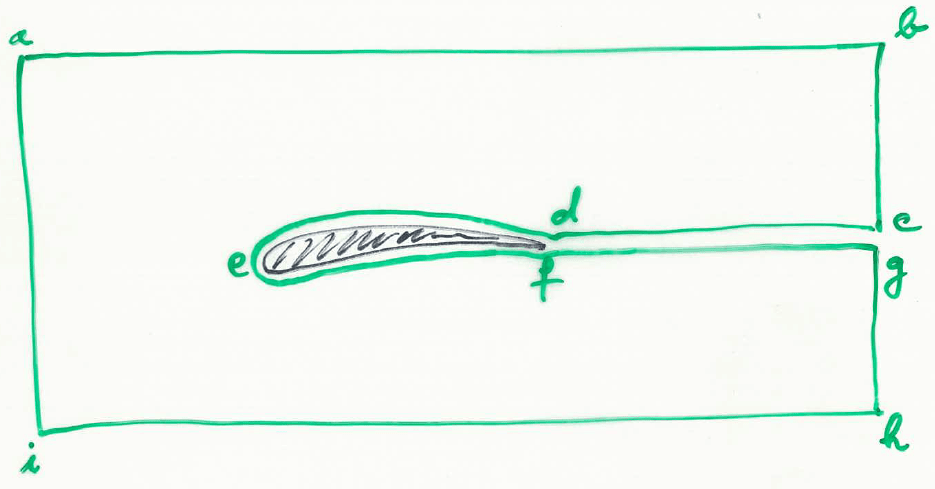
\includegraphics[scale=0.2]{ch1/1}
	\captionof{figure}{}
\end{wrapfigure}
When looking at an airfoil, we have a pressure that is applied around it. This pressure is non uniform, due to the presence of the airfoil. The integral of pressures over the surface gives a force expressed as the product of the incoming speed and the vorticity vector: the lift.

\subsection{Explain the origin of the bound vortex which exists around a profile which
	generates lift. Explain using the Kelvin theorem}
In inviscid case, the Kelvin theorem states that there cannot be vorticity, so no lift. If we take an arbitrary contour around the airfoil we will have no circultion. In inviscid case we can never get a lift $\rightarrow$ D’alembert paradox. At the trailing edge, if the flow wants to continue on the other corner from below, the velocity must be infinity so that the flow separates. But this is not the case in reality. \\

\begin{wrapfigure}[7]{r}{6.5cm}
	\vspace{-5mm}
	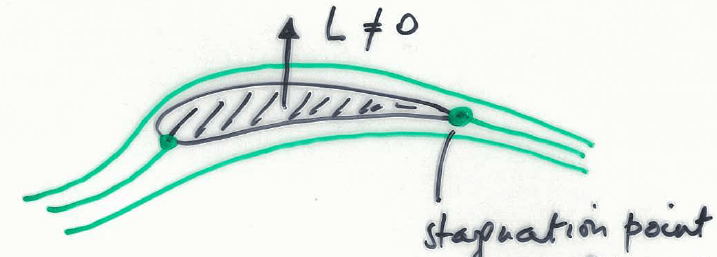
\includegraphics[scale=0.25]{ch1/4}
	\captionof{figure}{}\label{fig1}
\end{wrapfigure}
To satisfy the Kutta condition (the flow has to leave the airfoil smoothly), there needs to be circulation if we take a contour that contains the airfoil, but for all contour that does not contain the airfoil it is null.  $\Gamma$ varies with the stagnation point position, but only one corresponds to the Kutta condition. \\

\begin{wrapfigure}[16]{l}{4cm}
	\vspace{-5mm}
	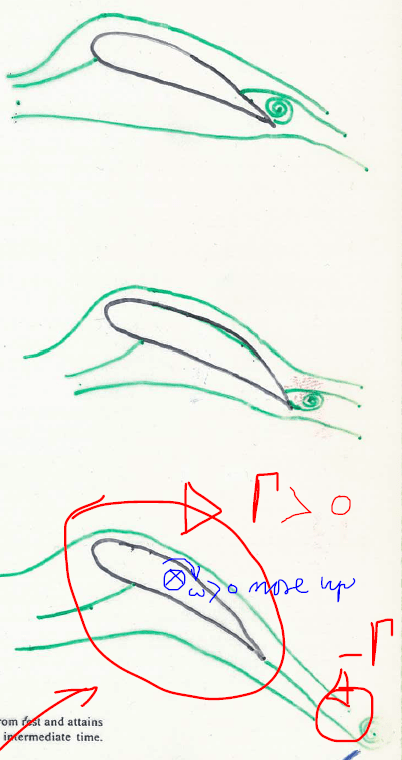
\includegraphics[scale=0.25]{ch1/5}
	\captionof{figure}{}
\end{wrapfigure}
The bound vortex is the vortex around the airfoil. It is compensated by a starting vortex that detaches from the airfoil.

We can show that every contour containing the airfoil has a non 0 circulation. Let's proof that a contour that doesn't contain the airfowl has $\Gamma =0$: 

\begin{equation}
\oint _{C} \vec{v}\, d\vec{l} = \oint _{\mbox{airfoil}} \vec{v}\, d\vec{l} + \oint _{cd} \vec{v}\, d\vec{l} + \oint _{fg} \vec{v}\, d\vec{l} = 0. 
\end{equation}

As the contour elements are exactly opposed to each other, the result is null. 

\subsection{What is the start-up vortex, what happens with it when the flow reaches a
	steady state}
What happens is that initially we have the first kind of flow, then the formation of the starting vortex due to viscous effects (separation) which is compensated by a \textbf{bound vortex} around the airfoil (to respect Kelvin theorem of irrotational flow) that makes $\Gamma \neq 0$. Then the vortex goes away to infinity. Indeed if we take $R = \rho v_\infty \Gamma$, $\Gamma \neq 0$, so we have lift. 
\subsection{Explain the Kutta condition}
The Kutta condition states that the flow can only have a stagnation point at the trailing edge. If this was not the case, the underwing flow would need to accelerate "going backwards" to meet the upperwing flow, see figure~\ref{fig1}.

%-----------------------------------------------------------------------------------------------------------------
%-----------------------------------------------------------------------------------------------------------------
%-----------------------------------------------------------------------------------------------------------------

\section{Derive an expression for the aerodynamic lift of on airfoil for inviscid
	incompressible flow (i.e. neglecting viscous effects).}

\begin{wrapfigure}[9]{l}{7.5cm}
	\vspace{-5mm}
	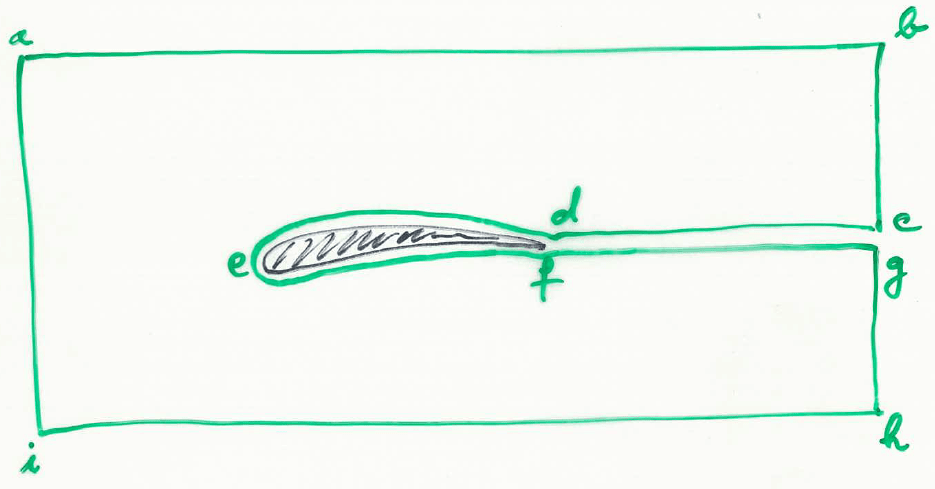
\includegraphics[scale=0.2]{ch1/1}
	\captionof{figure}{}
\end{wrapfigure}

The fundamental integral form of the mass conservation equation is:\\

\begin{equation}
\frac{d}{dt}\int _V \rho \, dV + \oint _S \rho \vec{v} \, d\vec{S} = 0.
\end{equation}

By applying Gauss theorem $\oint _S \vec{a}.\vec{n}\, dS = \int _V \nabla\vec{a}\, dV$:

\begin{equation}
\int _V \left[\frac{d \rho}{d t} + \nabla .(\rho \vec{v})\right]\, dV = 0. 
\end{equation}

True for all volumes:

\begin{center}
	\theor{
		\textbf{Continuity equation}
		\begin{equation}
		\frac{d \rho}{d t} + \nabla .(\rho \vec{u}) = 0
		\label{eq:1.3}
		\end{equation}
	}		
\end{center}

General form of the momentum equation is: 

\begin{equation}
\rho \dot{\vec{v}} = \frac{\D \rho \vec{v}}{\D t} + \rho (\vec{v}\nabla ) \vec{v} = -\nabla p + \nabla \bar{\bar{\tau}}.
\end{equation}

Steady state, time derivative goes away. If we consider the x component of the velocity, we can expend the derivative to the whole left term as:

\begin{equation}
\rho (\vec{v}\nabla ) v_x = \nabla (\rho \vec{v} v_x) - v_x \cancel{\nabla (\rho \vec{v})}
\label{eq:1.5}
\end{equation}

where the last term is null related to \eqref{eq:1.3} in steady state. Integrating both sides around the volume contained in the closed surface S (abcdefghi on figure) in \eqref{eq:1.5}, and applying Gauss theorem, we obtain:

\begin{equation}
\oint _{S} \vec{v} (\rho \vec{v} \vec{n}) \, dS = -\oint _{S} p \, d\vec{S} + \oint _{S} \bar{\bar{\tau}} \, d\vec{S}.
\label{eq:1.6}
\end{equation}		 

New closed contour $S* = S - \mbox{airfoil} - cd - fg$ (previous abhi in fact). \eqref{eq:1.6} becomes:

\begin{equation}
\begin{aligned}
&\oint _{S^*} \vec{v} (\rho \vec{v} \, d\vec{S})  + \cancel{\oint _{\mbox{airfoil}} \vec{v} (\rho \vec{v} \, d\vec{S})} + \cancel{\oint _{cd+fg} \vec{v} (\rho \vec{v} \, d\vec{S})} 
\\&= -\oint _{S^*} p \, d\vec{S} -\oint _{\mbox{airfoil}} p \, d\vec{S}-\cancel{\oint _{cd + fg} p \, d\vec{S}}+ \oint _{S^*} \bar{\bar{\tau}} \, d\vec{S} +\oint _{\mbox{airfoil}} \bar{\bar{\tau}}\, d\vec{S} +\cancel{\oint _{cd + fg} \bar{\bar{\tau}}\, d\vec{S}}
\end{aligned}
\label{eq:1.7}
\end{equation}

Forces applied to a wing:
\begin{equation}
\vec{R} = \oint _{\mbox{airfoil}} p\, d\vec{S} - \oint _{\mbox{airfoil}} \bar{\bar{\tau}}\, d\vec{S}	
\end{equation}

\begin{equation}
\oint _{S^*} \vec{v} (\rho \vec{v} \, d\vec{S}) = -\oint _{S^*} p \, d\vec{S} + \cancel{\oint _{S^*} \bar{\bar{\tau}} \, d\vec{S}} - \vec{R}.
\label{eq:1.9}
\end{equation}

Pressure effects induced by the body remains at a long distance from the body. We have to analyse the \textbf{non uniform} p along S*. In order to apply Bernouilli equation $p + \frac{1}{2}\rho v^2 = cst$, let's add the constants $p_\infty$ and $v_\infty$ to \eqref{eq:1.9}, as $\oint p_\infty\, d\vec{S} = p_\infty \oint d\vec{s} = 0$: 

\begin{equation}
\vec{R} = -\oint _{S^*} (p-p_\infty) \, d\vec{S} - \oint _{S^*} (\vec{v}-\vec{v}_\infty) \, d\dot{m}
\label{eq:1.12}
\end{equation}

Let's express $\vec{v} = \vec{v}_\infty + \vec{\delta _c}$ with $\vec{\delta _c}$ a perturbation. Introducing this in Bernouilli equation: 

\begin{equation}
\begin{aligned}
p_\infty +\frac{1}{2} \rho \cancel{\vec{v}_\infty ^2} = p + \frac{1}{2} \rho( &\vec{v}_\infty + \vec{\delta _c})^2 = p + \frac{1}{2} \rho (\cancel{\vec{v}_\infty ^2} + 2 \vec{v}_\infty \vec{\delta _c} + \cancel{\vec{\delta _c}^2}) \\
&\Rightarrow p-p_\infty = - \rho\vec{v}_\infty \vec{\delta _c}	.		
\end{aligned}
\end{equation}

If we replace this result in \eqref{eq:1.12}, we find:

\begin{equation}
\vec{R} =\oint _{S^*} \rho [(\vec{v}_\infty \vec{\delta _c}) \, d\vec{S} - \vec{\delta _c} [(\vec{v}_\infty . d\vec{S})]
\end{equation}

by using a vector property $\vec{a} \times (\vec{b} \times \vec{c}) = (\vec{a} \vec{b})\vec{c} - (\vec{a}\vec{c})\vec{b}$:

\begin{equation}
= \rho \vec{v}_\infty \times \oint _{S^*} \vec{\delta _c} \times d\vec{S} = \rho \vec{v}_\infty \times \left[\oint _{S^*} \vec{v} \times d\vec{S} - \cancel{\oint _{S^*} \vec{v}_\infty \times d\vec{S}}\right]
\end{equation}

and by applying Stokes theorem $\oint _S \vec{a} \times d\vec{S} = \int _V \nabla \times \vec{a} \, dV$:

\begin{equation}
= \rho \vec{v}_\infty \times \int  (\nabla \times \vec{v})\, dV = \rho \vec{v}_\infty \times \int  \vec{\omega}\, dV
\end{equation}

where $\vec{w}$ is the \textbf{vorticity vector} of direction $\vec{1}_z$ (pointing in the paper):

\begin{equation}
\vec{\omega} = 
\left| \begin{array}{ccc}
\vec{1}_x & \vec{1}_y & \vec{1}_z \\ 
\D _x & \D _y & 0 \\ 
v_x & v_y & 0
\end{array} 
\right| 
= [\D _x v_y - \D _y v_x] \vec{1}_z
\end{equation}

This shows that the lift force is always perpendicular to the flow!


\subsection{Express conservation of momentum over a closed surface S far away from
	the wing, neglecting viscous forces}
\begin{wrapfigure}[11]{l}{6.5cm}
	\vspace{-5mm}
	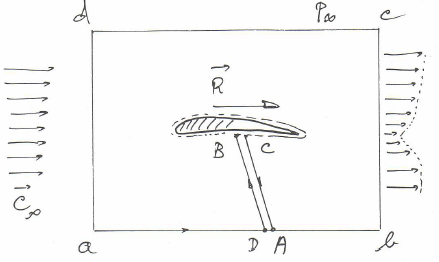
\includegraphics[scale=0.4]{ch1/2}
	\captionof{figure}{}
\end{wrapfigure}
By considering this (assumption of far field), we can compute the force only by knowing the far field parameters. Indeed, uniform pressure implies null surface integral, so that \eqref{eq:1.9} becomes:

\begin{equation}
\vec{R} = -\oint _{S^*} \vec{v} (\rho \vec{v} \, d\vec{S}).
\end{equation}

The velocity term remains, as by experience we know that there is a \textbf{wake} making the velocity profile non-uniform. Let's now consider that the velocity is horizontal so that $\vec{R} = R.\vec{1}_x$, at the inlet we have $\vec{v}$ and $\vec{n}$ are opposed while at the outlet they are in the same direction: 

\begin{equation}
\vec{R} = \int _a^d \vec{v}\, d\dot{m} - \int _b^e \vec{v}\, d\dot{m} > 0
\end{equation}

showing that there is only \textbf{drag} force.

\subsection{Show that the lift force is linked to the vorticity through the closed surface S}
See above.
\subsection{Show that for the 2D airfoil the lift force is linked to the circulation around
	the airfoil, derive the Kutta-Joukowski formula for the lift generated by a 2D
	profile}

We will now introduce the circulation $\Gamma = - \oint \vec{v} \, d\vec{l} >0$   around a body. The convention is to take the anticlockwise direction for $d\vec{l}$ and so for $\Gamma$ to be $>0$ we must have $\vec{v}$ in the clockwise direction. There is a link between the lift force and the circulation. Let's introduce \textbf{Stokes theorem}:

\begin{equation}
\oint \vec{a} d\vec{l} = \int _S (\nabla \times \vec{a})\, d\vec{S} \qquad \Rightarrow -\Gamma = \int _S \vec{\omega} d\vec{S}.
\end{equation}

We remember that:
\begin{equation}
\begin{aligned}
\vec{R} &= \rho \vec{v}_\infty \times \int  \vec{\omega}\, dV = \rho \vec{v}_\infty \times \int  l\vec{\omega}\, dS \qquad \Leftrightarrow \frac{\vec{R}}{l} = \rho \vec{v}_\infty \times \int  \vec{\omega}\, dS \\
\frac{\vec{R}}{l}&= \rho \vec{v}_\infty \times \int  \vec{\omega}\, (d\vec{S}.\vec{1}_z) = \rho \vec{v}_\infty \times (-\Gamma)\vec{1}_z = \rho v_\infty \Gamma \,\vec{1}_y
\end{aligned}
\end{equation}

to finally obtain a very good approximation of the lift:

\begin{center}
	\theor{
		\textbf{Kutta formula for lift 2D airfoil}
		\begin{equation}
		|R| = \rho v_\infty \Gamma 
		\end{equation}
	}
\end{center}


%-----------------------------------------------------------------------------------------------------------------
%-----------------------------------------------------------------------------------------------------------------
%-----------------------------------------------------------------------------------------------------------------

\section{Characteristics of a 2D airfoil:}
\subsection{Define lift and drag, give the principle components of lift and drag force in
	normal operation and in case of separation}
	
\begin{wrapfigure}[9]{l}{7.5cm}
	\vspace{-5mm}
	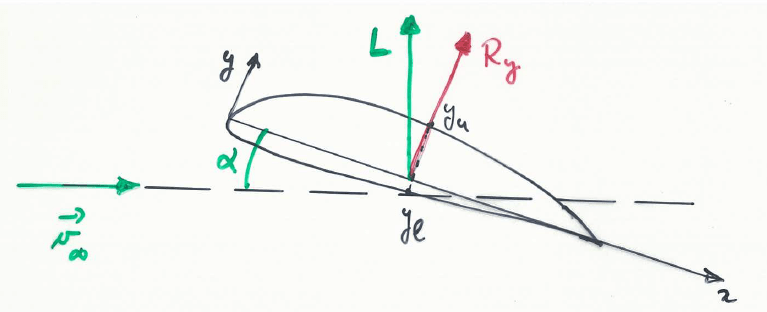
\includegraphics[scale=0.25]{ch2/3}
	\captionof{figure}{}
	\label{fig:2.2}
\end{wrapfigure}
Force applied on the wing:

\begin{equation}
\vec{R} = -\oint p \, d\vec{S} + \oint \bar{\bar{\tau}} \, d\vec{S} 
\end{equation}

with an external normal to the airfoil. The angle of attack is represented on \autoref{fig:2.2}.

The pressure term is responsible for lift and the friction term is responsible for drag. Friction forces work tangential to the airfoil and the pressure forces are perpendicular, if there is \textbf{no separation} in the flow. The drag created by the stress is called the \textbf{skin} or \textbf{friction} drag. 
Note that in a subsonic inviscid incompressible flow, we have the paradox of d’Alembert because we have no drag. This shows that the pressure only contributes to lift. \\

\textbf{Separation}: region above the airfoil where $p-p_\infty \approx 0$ $\Rightarrow$high pressure below $p\gg p_\infty$ that slows down the wing. This implies that the applied force is higher than the case without separation and due to the attack angle, the drag force too. This phenomenon is called \textbf{pressure drag} (form drag), and here the pressure contributes to drag.


\subsection{Explain the non-dimensional force coefficients($C_l$, $C_d$, $C_m$) and which are the
	similarity parameters influencing these coefficients}
Let’s look to the non-dimensional parameters that will influence the lift, the drag and the momentum. We have to define some reference quantities: 

\begin{equation}
\begin{array}{cccc}
L_{ref} = C & v_{ref} = v_\infty & t_{ref} = L_{ref}/v_{ref} & \rho _{ref} = \rho _\infty \\
t’= t/t_{ref} & p_{ref} = \rho _{ref} \frac{v_{ref} ^2}{2} & \mbox{Mach} = V_{ref} / a_{ref} & a_{ref} = \gamma \pi T_{ref} \\
\gamma = c_p / c_v && Re_{ref} = \frac{\rho _{ref} v_{ref} L_{ref}}{\mu _{ref}} &
\end{array}
\end{equation}					

where $a$ is the speed of sound. By replacing all these in the mass, momentum and energy equations, we obtain the non-dimensional ones (see Fluid Mechanics II):

\begin{equation}
\begin{aligned}
&\bullet\frac{\D \rho '}{\D t'} + \nabla \left(\rho ' \vec{v}'\right) = 0\\
&\bullet\rho ' \frac{d\vec{v}'}{dt'} = - \frac{1}{\gamma M^2_{ref}}\nabla p' + \frac{1}{\mbox{Re}_{ref}}\nabla \bar{\bar{\tau}'}\\
&\bullet\frac{d}{dt'}(\rho ' e')+ \frac{\gamma (\gamma -1)}{2} M^2_{ref}\frac{d}{dt'}(\rho ' \vec{v'}^2 ) \\
&= \frac{\gamma}{Pr_{ref}Re_{ref}} \nabla (k'\nabla T') - (\gamma -1)\nabla (p'\vec{v}')+ \gamma (\gamma -1) \frac{M_{ref}^2}{Re_{ref}} \nabla (\bar{\bar{\tau}}'\vec{v}')			\end{aligned}
\end{equation}

We can see that a solution can only be function of 4 parameters: $M, Re, Pr = \frac{c_p \mu}{k}, \gamma$, but we know that the geometry and the angle of attack $\alpha$ have a role by means of the boundary conditions. Then, we assume that the fluid is air ($\gamma =1.4$) and that we can neglect heat effects (no influence of Pr, incompressible and so low speed flows). The non-dimensional lift, drag and moment are thus function of M, Re, geometry and $\alpha$. We can define \textbf{lift}, \textbf{drag} and \textbf{moment coefficient} as (we forget about compressibility $\rightarrow$ M, and Re effects are low for $C_L and C_M$): 

\begin{equation}
\begin{aligned}
&C_L(\cancel{M}, \cancel{Re}, geometry, \alpha) = \frac{L}{\frac{1}{2}\rho _{ref} v^2_{ref} S} \\
&C_D(\cancel{M},Re, geometry, \alpha) = \frac{D}{\frac{1}{2}\rho _{ref} v^2_{ref} S}		\\
&C_M(\cancel{M}, \cancel{Re}, geometry, \alpha) = \frac{M}{\frac{1}{2}\rho _{ref} v^2_{ref} Sc}
\end{aligned}	
\label{eq:2.18}		
\end{equation}

where L, D, M are the \textbf{dimensional} forces, c the mean chord (S/b) and S a reference surface (3D wing $\rightarrow$ total wing surface, 2D wing $\rightarrow$ S = c). We can experimentally show that the lift increases mainly linearly with $\alpha$ and the drag force is caused by friction effects and pressure differences involving with $\alpha$. This gives the following equations (lower case for 2D):

\begin{equation}
c_l = m(\alpha - \alpha _{L_0}) \qquad c_d = c_{d_0} + kc^2_l
\end{equation}

where $m\approx 2\pi$ theoretically and 5.7 practically, k is a constant of order of magnitude 0.01.

\subsection{Explain:}
\textbf{center of pressure CP:} It's the x value on the chord where the carrier of the force $\vec{R}$ intersects the chord. It's function of the angle of attack. Indeed, if alpha increases, the suction peak will be higher, this induces that the center of pressure move forward (participation of the forward pressure more important).\\

Note that the center of pressure is not a fixed point. Indeed, it varies with the angle of attack: if $\alpha \nearrow$, the pressure peak on the LE is more important making the $x_p$ move upstream, and the contrary for $\alpha \searrow$. This notion will be completed by the \textbf{zero lift angle} $\alpha _{0}$.

\textbf{equivalent force system in an arbitrary point Q on the chord of the profile:} 
\begin{wrapfigure}[7]{l}{3cm}
	\vspace{-5mm}
	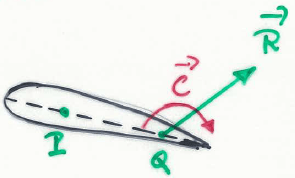
\includegraphics[scale=0.3]{ch2/11}
	\captionof{figure}{}
\end{wrapfigure}
The force at the pressure center P is equivalent to another force in point Q, but by adding the moment to compensate the one added by moving the force. This moment is:

\begin{equation}
\vec{C_Q} = -\vec{PQ}\times \vec{R}.
\end{equation}
\textbf{aerodynamic center AC:} Suppose that there is a point Q where the couple $C_Q$ is independent of the angle of attack (because the pressure center changes with alpha). This point is called the aerodynamic center.

The moment at this point is always nose-down and the point is situated upstream to the center of pressure.

\textbf{the graph of the momentum coefficient $c_m$ at a point Q versus the
	lift coefficient $c_l$ for Q located at the trailing edge, at the leading edge and at
	the aerodynamic center of the profile:} It is shown experimentally that:

\begin{equation}
c_m(Q) = c_{m_0} + k c_l
\label{eq:2.11}
\end{equation}

\begin{center}
	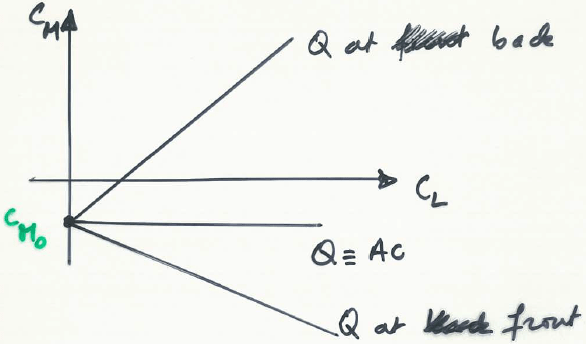
\includegraphics[scale=0.23]{ch2/14}
	\captionof{figure}{}
\end{center}
$k$ is a constant that is related to the reference point chosen. If $Q$ is taken on the LE for example, increasing $\alpha$ will produce an increase of the lift and make the center of pressure move upstream. The L increase will compensate the moving $x_p$ such that the moment becomes even more noose-down (more negative following $\vec{1}_z$) $\Rightarrow k<0$ for a decrease in \eqref{eq:2.11}. The same reasoning applied on the trailing edge gives $k>0$. 
\subsection{Compute the Location of the center of pressure CP as a function of the angle of
	attack alpha}
\begin{equation}
\begin{array}{cccc}
1) & c_m = c_{m_0} + kc_l & 2)& M_{ac} = (x_{ac}-x_{cp})N \\
3) & m_{ac} = M_{AC} = M_0 <0 & 4) & N = n(\alpha-\alpha _0)
\end{array}
\end{equation}

The AC being always upstream the CP the difference in 2) is $<0$. In 4), $n>0$. By using equation 3,4 and 2, we can compute:

\begin{equation}
M_0 = -(x_{cp}-x_{ac}).n(\alpha - \alpha _0) \quad \Leftrightarrow \quad -\frac{M_0}{n} = (x_{cp}-x_{ac}).(\alpha - \alpha _0)
\end{equation}


\begin{wrapfigure}[8]{l}{4.5cm}
	\vspace{-5mm}
	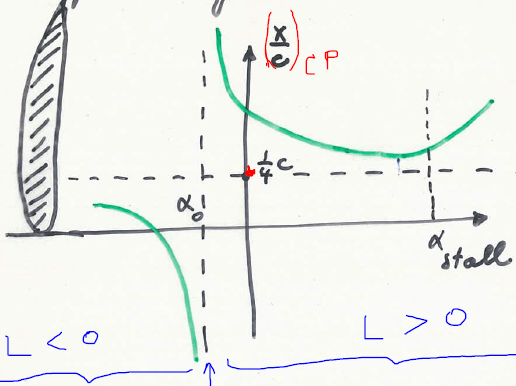
\includegraphics[scale=0.2]{ch2/17}
	\captionof{figure}{}
\end{wrapfigure}
This is the equation of an \textbf{hyperbola}. To see it, we only have to compute the limits of:

\begin{equation}
\begin{array}{c}
x_{cp} = x_{ac} - \frac{M_0}{n}\frac{1}{\alpha - \alpha _0}\\
\lim _{\alpha \rightarrow \pm\infty} x_{cp} = x_{ac} \qquad \lim _{\alpha \rightarrow \alpha _0 >0} x_{cp} = +\infty \qquad \lim _{\alpha \rightarrow \alpha _0 <0} x_{cp} = -\infty
\end{array}
\end{equation}

Let's finally say that commonly, $x_{ac} = cst \approx \frac{1}{4}C$.
\subsection{Explain the lift, drag and moment curves as a function of the angle of attack alpha}
Starting from what is said in 3.2, experiment showed that lift is increasing linearily with $\alpha$, and drag goes proportionnaly to $c_l^2$. The moment is proportionnal to $c_l$, we thus expect it to be linear with respect to $\alpha$.

\subsection{Explain what is stall and critical angle of attack. Explain different types of stall.}
\begin{wrapfigure}[11]{l}{6cm}
	\vspace{-5mm}
	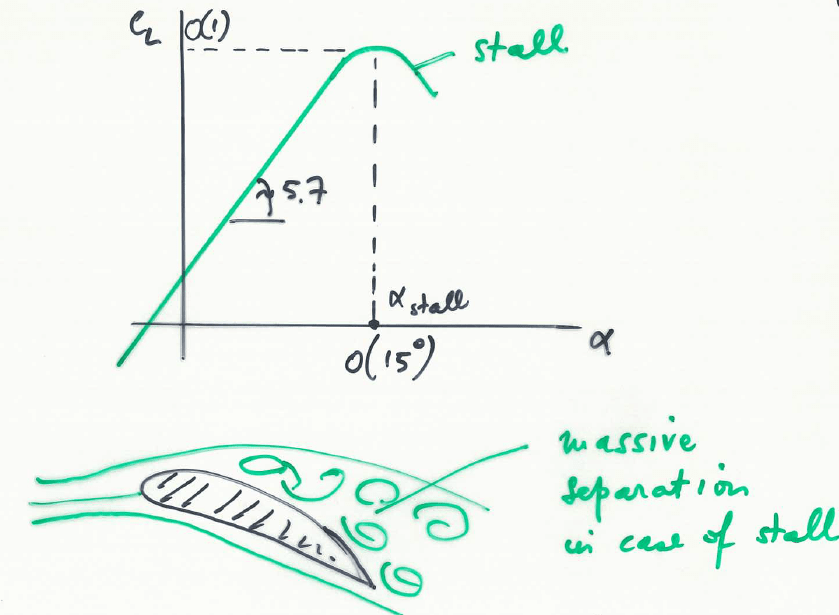
\includegraphics[scale=0.16]{ch2/18}
	\captionof{figure}{}
\end{wrapfigure}
At a certain angle of attack ($\approx 15\degres$), the lift suddenly drops. This is due to massive separation on the suction side (reverse pressure gradient too high) and happens at the \textbf{critical angle of attack}. This phenomenon is called \textbf{stall}. In the separated part, the pressure will no longer decrease and will form a pressure plateau. \\

We have to make the difference between leading-edge stall and trailing-edge stall. For \textbf{leading-edge stall}, the massive separation occurs suddenly near the LE resulting \newpage

\begin{wrapfigure}[13]{r}{5.7cm}
	\vspace{-5mm}
	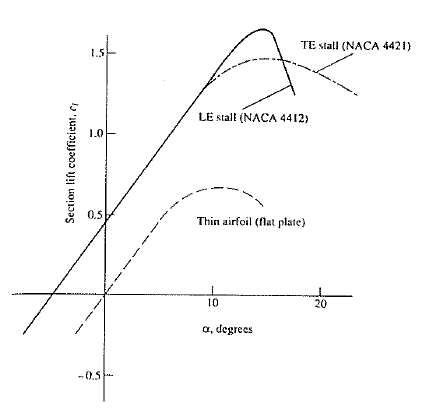
\includegraphics[scale=0.4]{ch2/19}
	\captionof{figure}{}
\end{wrapfigure}
in a strong and sudden drop of lift, when at maximum lift. This especially occurs to thin airfoils with cross-sections between 10 and 16\% of the chord. For the \textbf{trailing-edge stall}, the point of separation gradually goes upstream with increasing angle of attack resulting in a more gradual drop of lift (more thick airfoils). The comparison is done on the right figure. We can also see a third type of stall called \textbf{thin airfoil stall} with the example of a flat plat.  \\

In conclusion, the LE must be sufficiently rounded to have a good maximum lift. In fact the profile may nor be too 

\begin{wrapfigure}[8]{l}{7cm}
	\vspace{-5mm}
	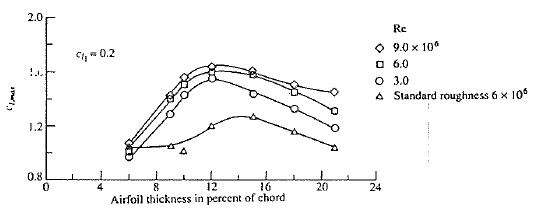
\includegraphics[scale=0.4]{ch2/20}
	\captionof{figure}{}
\end{wrapfigure}
thick  nor too thin. The figure on the left shows the influence of the thickness on the lift. We notice that the optimum thickness is situated around 12\% of the chord.The maximum lift increases with RE, indeed higher the Re, higher is the ratio of speed versus viscosity. So we can better oppose to separation. Unlike the Re number, the roughness has great effects on the maximum lift. Finally, let's notice that the camber have also an effect on maximum lift, the best is a camber of 8 up to 10\%.

\begin{equation}
L = C_L \frac{1}{2} \rho _{ref} v^2_{ref} S.
\label{eq:2.21}
\end{equation}

The lift force must always at least be equal to the weight of the plane. This implies that for low speed (take-off and landing), the $C_L$ must be large. This is accomplished with large $\alpha$ and slats or flaps. The minimum speed where the lift can still balance the weight ($C_L$ maximum) is called \textbf{stall speed} and from \eqref{eq:2.21} we find:

\begin{equation}
v_{stall} = \sqrt{\frac{W}{C_{L_{max}} \frac{1}{2} \rho_{ref} S}}
\end{equation}

\subsection{Discuss the polar curve of the airfoil, i.e. lift coefficient as a function of drag
	coefficient, show the glide ratio on this plot}
\begin{wrapfigure}[10]{r}{4cm}
	\vspace{-5mm}
	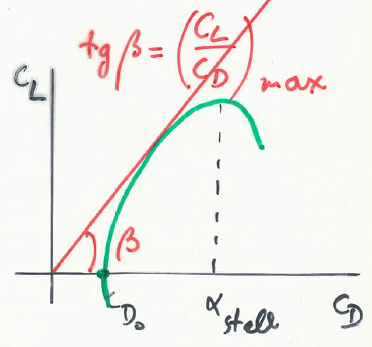
\includegraphics[scale=0.3]{ch2/21}
	\captionof{figure}{}
\end{wrapfigure}
The curve that represents $C_L$ in function of $C_D$ is the \textbf{polar curve} of the wing. The ratio $\frac{C_L}{C_D}$ is the \textbf{glide ratio} or \textbf{finesse} and is like an efficiency parameter. 
\subsection{What is the importance of the glide ratio, discuss the case of a gliding plane
	(engine off situation)}
The best parameter is obtained using the graph by calculating $\beta$ such that: 

\begin{equation}
\tan \beta = \left(\frac{C_L}{C_D}\right)_{max}
\end{equation}						

This point is important for the quality of the wing because if we plot the thrust, the lift, the drag and the weight of a plane describing a horizontal flight (\autoref{fig:2.21}), the thrust is given by:

\begin{equation}
T = \frac{L}{\tan \beta} = \frac{W}{\tan \beta}
\end{equation}

where we see that when $\tan \beta$ (so the glide ratio) increases, T decreases. Another interpretation can be given when we have no thrust (\autoref{fig:2.22}). In this case the gliding ratio has to be adapted to travel the larger distance knowing that:

\begin{equation}
\frac{C_L}{C_D} = \frac{\mbox{distance travelled}}{\mbox{height loss}}
\end{equation}

\begin{center}
	\begin{minipage}{0.3\textwidth}
		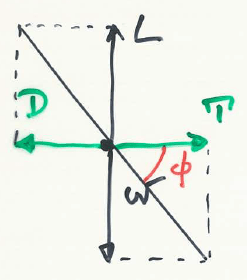
\includegraphics[scale=0.5]{ch2/22}
		\captionof{figure}{}			
		\label{fig:2.21}
	\end{minipage}
	\begin{minipage}{0.5\textwidth}
		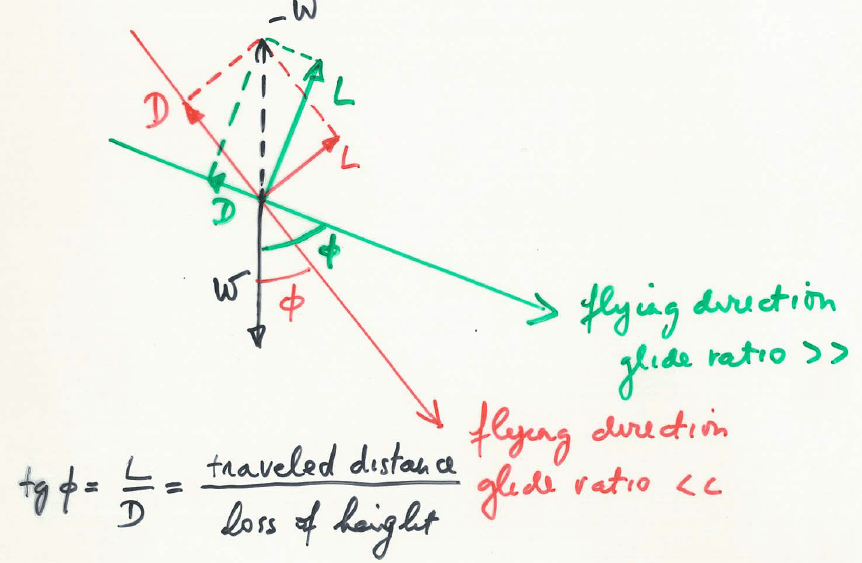
\includegraphics[scale=0.2]{ch2/23}
		\captionof{figure}{}			
		\label{fig:2.22}
	\end{minipage}
\end{center}
%-----------------------------------------------------------------------------------------------------------------
%-----------------------------------------------------------------------------------------------------------------
%-----------------------------------------------------------------------------------------------------------------

\section{Computation of inviscid irrotational flow around a 2D airfoil using conformal
	mapping - Joukowski profiles}
\subsection{Explain methods based on complex potential function, explain the
	connection with usual stream function and potential function}
We will begin here with steady, inviscid irrotational flows. This gives for the mass conservation equation:

\begin{equation}
\frac{\D \rho}{\D t} + \nabla (\rho \vec{v}) = 0 \qquad \Rightarrow \nabla \vec{v} = 0 = \D _x u + \D _y v
\end{equation}

In the other hand, we have the assumption of irrotational flow:

\begin{equation}
\vec{\omega} = 0 \qquad \Rightarrow \D _x v - \D _y u = 0.
\end{equation}

Then we define the \textbf{complex potential function w}:

\begin{equation}
w = \phi + I\psi
\end{equation}		 

where $\phi$ is the \textbf{potential function} (satisfies $w=0$ by construction) such that:

\begin{equation}
\left\{
\begin{aligned}
&u = \D _x \phi \\
&v = \D _y \phi
\end{aligned}
\right.
\qquad
\nabla \phi = \vec{v} = \D _x\phi \vec{1} _x + \D _y \phi \vec{1}_y
\end{equation}

We must satisfy the mass conservation equation:
\begin{equation}
\nabla (\nabla \phi) = 0 \qquad \Rightarrow \Delta \phi = 0 
\end{equation}

coupled with boundary conditions, we can find a solution $\phi (x,y)$. The \textbf{stream function} satisfies the mass conservation by construction:

\begin{equation}
\left\{ 
\begin{aligned}
&u = \D _y \psi\\
&v = - \D _x \psi
\end{aligned}
\right.
\qquad \Rightarrow \D _x u + \D _y v = 0 \Leftrightarrow \D _x (\D _y \psi) + \D _y (- \D _x \psi) = 0
\end{equation}

\begin{wrapfigure}[8]{l}{4cm}
	\vspace{-5mm}
	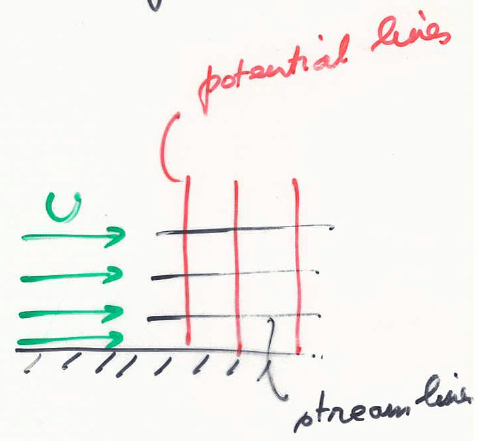
\includegraphics[scale=0.2]{ch2/24}
	\label{fig:2.23}
	\captionof{figure}{}
\end{wrapfigure}
We still have to verify the $\omega=0$ condition:
\begin{equation}
\D _x v - \D _y u = 0 \qquad \Rightarrow \frac{\D ^2 \psi}{\D x^2} + \frac{\D ^2 \psi}{\D y^2} = 0 \qquad \Delta \psi = 0
\end{equation}
A streamline and a potential line are perpendicular to each other:
\begin{equation}
\nabla \psi . \nabla \phi = \D _x \psi \D _x \phi + \D_ y \psi \D _y \phi = -vu + uv = 0. 
\end{equation}

	Analytical means differentiable. This consist in defining a function $f(z)$ analytical such that:

\begin{equation}
w = f(z) \qquad z,\omega \in \mathbb{C} \qquad \Rightarrow w = \phi +i \psi \qquad \left\{
\begin{aligned}
&z= x+iy\\ 		 
&\phi = \phi (x,y) \in \mathbb{R}\\
&\psi =  \psi(x,y) \in \mathbb{R}
\end{aligned} 		  
\right.
\end{equation}

If this is differentiable everywhere, $\Delta \phi = \Delta \psi = 0$. 

\subsection{Explain how the velocity can be computed from the complex potential
	function}

The complex velocity (velocity field):

\begin{equation}
\frac{dw}{dz} = \frac{df}{dz} = A + iB \qquad A = \frac{\D \phi}{\D x} = - \frac{\D \psi}{\D y} = u \quad B = \frac{\D \psi}{\D x} = - \frac{\D phi}{\D y} = -v
\end{equation}

A property of this $f(z)$ is the superposition principle: $w_1 = f_1(z), w_2 = f_2(z)$ so $w_1 + w_2 = f_1(z)+f_2(z)$.
\subsection{Derive the complex potential function for uniform flow, source/sink flow,
	free vortex}
\subsubsection{Uniform flow}

\begin{equation}
w = U z \qquad \frac{d w}{dz} = U = u+iv \qquad \Rightarrow u = U; v = 0
\end{equation}

\subsubsection{Source / Sink}
\begin{wrapfigure}[8]{r}{3cm}
	\vspace{-5mm}
	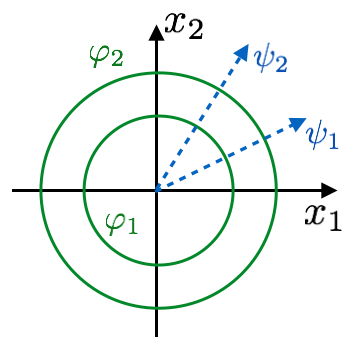
\includegraphics[scale=0.3]{ch2/25}
	\captionof{figure}{}
\end{wrapfigure}
In this case, using the cylindrical coordinates, the complex potential is defined as ($\Lambda$ being the volumetric flow): 

\begin{equation}
\begin{aligned}
&w = \frac{\Lambda}{2\pi} \ln z = \frac{\Lambda}{2\pi} \ln (r e^{i\theta}) = \frac{\Lambda}{2\pi} (\ln r + i\theta) \\
&\Rightarrow \phi = \frac{\Lambda}{2\pi} \ln r, \psi =  \frac{\Lambda}{2\pi}\theta.
\end{aligned}
\end{equation}

We see that complex lines corresponds to $r =cst$ so are circles and streamlines $\theta = cst$ are line of constant angle. $\oint \vec{v}\, d\vec{l}=0$ as velocity is everywhere tangent to any circular contour. Let's compute the derivative for the velocity field:

\begin{equation}
\frac{dw}{dz} = \frac{\Lambda}{2\pi z} = \frac{\Lambda (x-iy)}{2\pi (x^2+y^2)} = \frac{\Lambda}{2\pi r} (\cos \theta - i \sin \theta).
\end{equation}

We see that the velocity decreases in $1/r$, this is due to the constant mass flow, so if the surface increases with r the velocity has to decrease to keep $\dot{m} = \rho v S$ constant. 

\subsubsection{Free vortex}
\begin{wrapfigure}[5]{l}{3cm}
	\vspace{-5mm}
	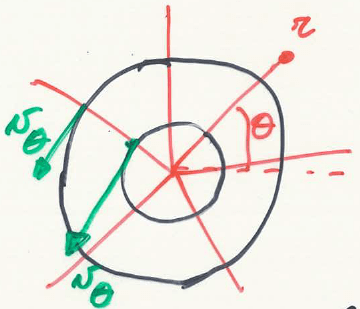
\includegraphics[scale=0.23]{ch2/26}
	\captionof{figure}{}
\end{wrapfigure}
We do the same as the other cases: 
\begin{equation}
\begin{aligned}
&w = \frac{i\Gamma}{2\pi} \ln z = \frac{i\Gamma}{2\pi} \ln (re^{i\theta}) = \frac{i\Gamma}{2\pi} (\ln r + i\theta) = -\frac{\Gamma}{2\pi} \theta + \frac{i\Gamma}{2\pi} \ln r \\
&\phi = -\frac{\Gamma}{2\pi} \theta, \psi = \frac{\Gamma}{2\pi} \ln r
\end{aligned}
\end{equation}

We see that this is the inverse case of the previous one, streamlines are circles oriented in negative rotational motion around z-axis (z entering in the sheet) so clockwise. We can compute the velocity field by deriving among z and we find that: 

\begin{equation}
u = \frac{\Gamma \sin \theta}{2 \pi r} \qquad v = -\frac{\Gamma \cos \theta}{2\pi r}
\end{equation}

Let's specify that $v_\theta = \frac{1}{r} \frac{\D \phi}{\D \theta} = -\frac{\Gamma}{2 \pi r}$, and that we have a vortex singularity in the center because $\Gamma = 0. \infty$.

\subsection{Compute flow around Rankine body and around a cylinder}

	\begin{wrapfigure}[5]{r}{5.5cm}
	\vspace{-5mm}
	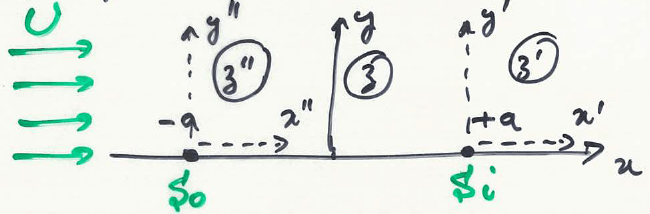
\includegraphics[scale=0.23]{ch2/27}
	\captionof{figure}{}
\end{wrapfigure}
Let's make a combination of a uniform flow and a source + sink as shown on the figure. The combination gives:

\begin{equation}
w = Uz + \frac{\Lambda}{2\pi} \ln \frac{z+a}{z-a}= Uz + \frac{\Lambda}{2\pi} \ln \frac{1+a/z}{1-a/z}.
\end{equation}

To have the flow around a cylinder we need to compute the limit $a\rightarrow 0$, and will need the Taylor expansion of $\ln$:

\begin{equation}
\ln \frac{1+\epsilon}{1-\epsilon} \approx 2 \epsilon + \cancel{o(\epsilon ^3)} \qquad \Rightarrow \lim _{a\rightarrow 0} w = \lim _{a \rightarrow 0} \left[ Uz + \frac{\Lambda}{2\pi} 2 \frac{a}{z} \right]
\end{equation}

by defining $\mu = 2\Lambda a$ we find the \textbf{flow around a cylinder}:

\begin{equation}
w = Uz + \frac{\mu }{2\pi z}.
\label{eq:2.42}
\end{equation}

If we replace $z= x+iy$ to find $\phi$ and $\psi$ we find:

\begin{equation}
\phi = Ux + \frac{\mu}{2\pi }\frac{x}{r^2} \qquad \psi = Uy - \frac{\mu }{2\pi} \frac{y}{r^2}.
\end{equation}

In this flow a closed streamline exists forming the so called \textbf{Rankine body} and which describes a cylinder in the case $a\rightarrow 0$. Indeed it is possible to find an exact solution for $\psi = 0$. This configuration has a symmetry according to x and y-axis when taking the center of the cylinder as origin. This implies that $\vec{F} = - \oint _{cyl} p\, d\vec{S} = 0$. This is the so called \textbf{paradox of d'Alembert} because we expect to find at least a drag force. A lift force can be find on the cylinder by adding a vortex. We conclude by saying that we can rewrite \eqref{eq:2.42} as (R the radius of the cylinder):

\begin{equation}
w = U\left( z + \frac{R^2}{z} \right) \qquad with \ R^2 = \frac{\mu }{2\pi U}.
\end{equation}

\subsection{Explain how a the class of Joukowski profiles is obtained by conformal
	mapping of a circle}
\begin{wrapfigure}[5]{l}{5.5cm}
	\vspace{-5mm}
	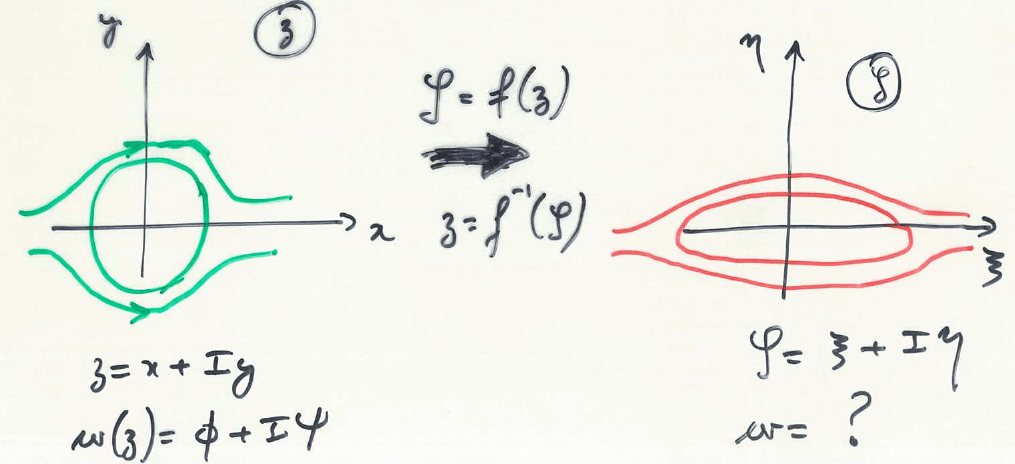
\includegraphics[scale=0.1]{ch2/28}
	\captionof{figure}{}
\end{wrapfigure}
Let's do a mapping, a transformation, to try to find our airfoil based on simple geometries. Let's as first example apply the transformation $Z = z + \frac{R^2}{z}$ to the cylinder of radius R. Let's first remark that the cylinder will become a flat plate:

\begin{equation}
Z = z + \frac{R^2}{z} = Re^{i\theta}  \frac{R^2}{Re^{i\theta}} = 2 R \cos \theta 
\end{equation}

Indeed, as $\cos \theta \in [-1,1]$ and the result is real, we have a flat plate between -2R and 2R in the x-axis. The flow Z is directly found: $W(Z) = UZ$. The second example will be the application of the same transformation on a cylinder of this time radius $r>R$. In this case the circle becomes an ellipse:

\begin{equation}
Z = r e^{i\theta} + \frac{R^2}{r^2}e^{-i\theta} = \left( r + \frac{R^2}{r} \right)\cos \theta + i \left( r - \frac{R^2}{r} \right) \sin \theta.
\end{equation}		 

Let's also compute the velocity field using the chain rule:

\begin{equation}
\frac{dW}{dZ} = \frac{dw}{dZ} = \frac{dw}{dz}\frac{dz}{dZ} = \left( 1 -\frac{r^2}{z^2} \right) \left( \frac{1}{1-\frac{R^2}{z^2}} \right).
\end{equation}

We see that the expression becomes infinite when $z^2 = R^2$. The reason is that the transformation is not analytical in these points so they must not be in the flow. 

The examples are summarized in the figures below 

\begin{center}
	\begin{minipage}{0.45\textwidth}
		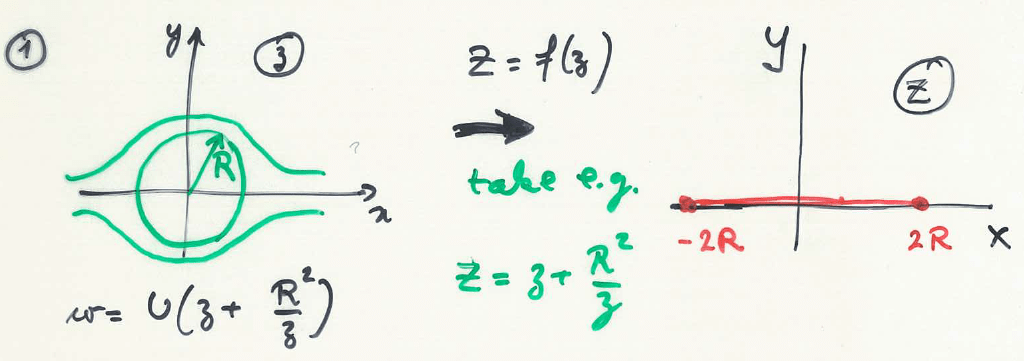
\includegraphics[scale=0.15]{ch2/29}
		\captionof{figure}{}
	\end{minipage}
	\begin{minipage}{0.45\textwidth}
		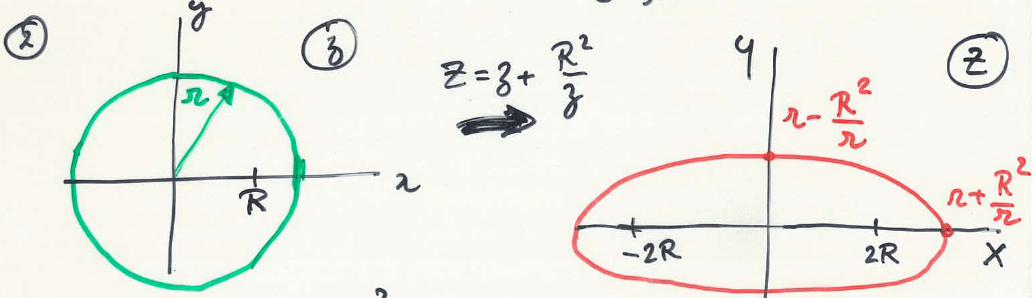
\includegraphics[scale=0.2]{ch2/30}
		\captionof{figure}{}
	\end{minipage}
\end{center}

Now suppose that we place no longer the center of the cylinder at the origin, but on the real axis. The mapping of the cylinder now takes the shape of a \textbf{symmetrical wing profile}. We see that there is two remarkable points that are H and A corresponding to the points $H_1$ and $A_1$ of the black and red circles, our profile is in between them. Now to give camber we only have to move the center of the cylinder on the y-axis. Please reffer to figures below. 

\begin{center}
	\begin{minipage}{0.45\textwidth}
		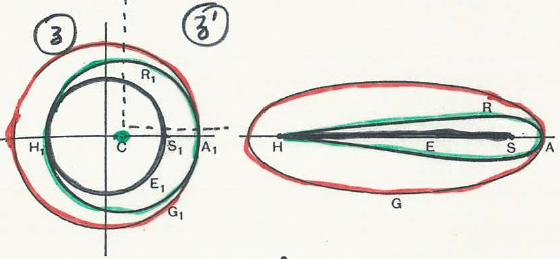
\includegraphics[scale=0.3]{ch2/31}
		\captionof{figure}{}
	\end{minipage}
	\begin{minipage}{0.45\textwidth}
		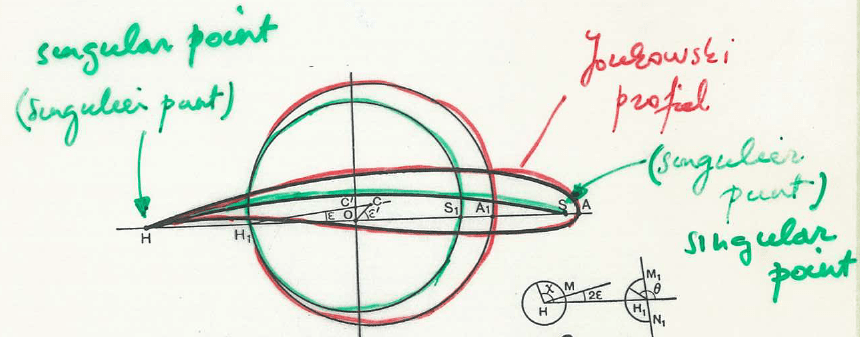
\includegraphics[scale=0.2]{ch2/32}
		\captionof{figure}{}
	\end{minipage}
\end{center}

Note that for the green circle in first figure, the complex potential becomes:

\begin{equation}
w = U\left( z-z_c + \frac{r^2}{z-z_c} \right)
\end{equation}

As last remark, let's remind that we had singularities in the second example. These points corresponds here to $H_1$ and $S_1$. The mapping of $H_1$ is always H the trailing edge, the velocity is there infinitely large. This was the discussion we've previously done with the stagnation point that has to move on the trailing edge otherwise $v = \infty$ because of the sharp edge. We can solve this by adding a vortex. This methods gives a limited amount of airfoils.

%-----------------------------------------------------------------------------------------------------------------
%-----------------------------------------------------------------------------------------------------------------
%-----------------------------------------------------------------------------------------------------------------

\section{Computation of inviscid irrotational flow around a thin airfoil based on a
	continuous distribution of vortices}
\subsection{Explain what is a free vortex}

A free vortex is an irrotationnal vortex where the flow velocity u is inversely proportional to the distance r.
\begin{wrapfigure}[5]{l}{3cm}
	\vspace{-5mm}
	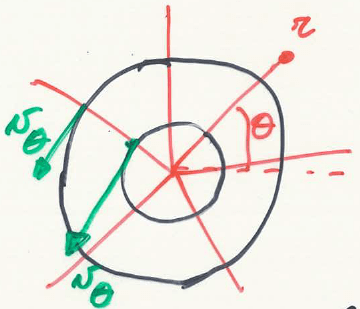
\includegraphics[scale=0.23]{ch2/26}
	\captionof{figure}{}
\end{wrapfigure}

Streamlines are circles oriented in negative rotational motion around z-axis (z entering in the sheet) so clockwise. We can compute the velocity field by deriving among z and we find that: 

\begin{equation}
u = \frac{\Gamma \sin \theta}{2 \pi r} \qquad v = -\frac{\Gamma \cos \theta}{2\pi r}
\end{equation}

Let's specify that $v_\theta = \frac{1}{r} \frac{\D \phi}{\D \theta} = -\frac{\Gamma}{2 \pi r}$, and that we have a vortex singularity in the center because $\Gamma = 0. \infty$.

\subsection{Explain what is a continuous distribution of free vortices on a line}
\subsection{Explain principle of the method of ree vortex distribution applied thin airfoils,
	limitations and hypotheses}
\subsection{Establish the integral equation which allows to compute the vortex
	distribution for a given profile}
\subsection{Show how to solve this equation using a spectral method, i.e. by expressing
	the vortex distribution as a truncated Fourier series}
\subsection{How is the Kutta-Youkowski condition imposed (allowing to compute the lift)}
\subsection{Starting from the expressions for the Fourier coefficients, compute the
	circulation and lift coefficient as a function of angle of attack, explain the
	result}
\subsection{Starting from the expression for the momentum coefficient at the leading
	edge $c_m$(LE), show that it’s a linear function of the lift coefficient $c_l$}
\subsection{Compute the location of the aerodynamic center AC and the momentum
	coefficient in the aerodynamic center}
\subsection{Compute the location of the center of pressure}

%-----------------------------------------------------------------------------------------------------------------
%-----------------------------------------------------------------------------------------------------------------
%-----------------------------------------------------------------------------------------------------------------

\section{title}
\subsection{title}
\subsection{title}
\subsection{title}

%-----------------------------------------------------------------------------------------------------------------
%-----------------------------------------------------------------------------------------------------------------
%-----------------------------------------------------------------------------------------------------------------

\section{title}
\subsection{title}
\subsection{title}
\subsection{title}

%-----------------------------------------------------------------------------------------------------------------
%-----------------------------------------------------------------------------------------------------------------
%-----------------------------------------------------------------------------------------------------------------

\section{title}
\subsection{title}
\subsection{title}
\subsection{title}

%-----------------------------------------------------------------------------------------------------------------
%-----------------------------------------------------------------------------------------------------------------
%-----------------------------------------------------------------------------------------------------------------

\section{title}
\subsection{title}
\subsection{title}
\subsection{title}

%-----------------------------------------------------------------------------------------------------------------
%-----------------------------------------------------------------------------------------------------------------
%-----------------------------------------------------------------------------------------------------------------

\section{title}
\subsection{title}
\subsection{title}
\subsection{title}

%-----------------------------------------------------------------------------------------------------------------
%-----------------------------------------------------------------------------------------------------------------
%-----------------------------------------------------------------------------------------------------------------

\section{title}
\subsection{title}
\subsection{title}
\subsection{title}

%-----------------------------------------------------------------------------------------------------------------
%-----------------------------------------------------------------------------------------------------------------
%-----------------------------------------------------------------------------------------------------------------

\section{title}
\subsection{title}
\subsection{title}
\subsection{title}




\end{document}